%EM on the probabilistic model + algorithm
\section{Experiments}
In this section, we try to evaluate the performance of the two models on different datasets. We first present the experimental setup and the datasets used for the experiments. We then present the results obtained for the estimation algorithms on synthetic data and on real-life datasets. We finally discuss the results obtained and the relevance of the models. 

The goal of these experiments is to compare the two models but also to individually test their ability to cluster ordinal datasets and to check whether they are able to generalize to real-life datasets. 

\subsection{Experimental setup}
\paragraph{Parameters of the experiment}
In this section, we propose to test the BOS model on synthetic data and on real-life datasets. 
To do so, we also use simple clustering algorithms to compare the performance of the BOS model on data that is adapted (ordinal) with algorithms that are not designed for this kind of data such as K-Means \citep{macqueen1967some} and Gaussian Mixture Models \citep{reynolds2009gaussian}.

We also test the AECM algorithm for the BOS model with both a random initialization of the parameters and an initialization of the parameters using the K-Means algorithm. \\ \\
Runtimes are also measured on the same machine for all the algorithms to compare their efficiency.
\paragraph{Dataset.} One of the main goal of the experiments is to test the ability of the models to generalize to real-life datasets. We therefore propose to test the illustrated methods on real world datasets to check the usefulness of the models on different real-life situations. Since the algorithm is specifically designed for ordinal observations, the datasets need to be adapted for the task. One way to apply to obtain real-life datasets is to quantize continuous datasets of observations that can be categorized (e.g. movies, store products, species...) \citep{skubacz2000quantization}. Another interesting approach could be to test the models on tasks that they were not specifically designed for. This could allow seeing how they can generalize and whether they are applicable to a broader class of problems. We therefore propose to test the ability to cluster observations of binary features into different animal species.
\paragraph{Zoo Dataset.} The zoo dataset consists of multiple features describing $101$ different animals, with most of them being binary variables associated to a characteristic of the animal (hair, feathers, eggs, milk, \ldots) \citep{misc_zoo_111}. Every animal belongs to one of $6$ classes. 
\paragraph{Car Evaluation Dataset.} The car evaluation dataset consists of multiple features describing $1728$ different cars, with most of them being ordinal variables associated to a characteristic of the car (buying price, maintenance price, number of doors, \ldots) \citep{misc_car_evaluation_19}. Every car belongs to one of $4$ classes.
\paragraph{Hayes-Roth Dataset.} The Hayes-Roth dataset consists of multiple features describing $132$ different persons, with most of them being binary variables associated to a characteristic of the person (has a PhD, is married, is a professional, \ldots) \citep{misc_hayes_roth_44}. Every person belongs to one of $3$ classes.
\paragraph{Caesarian Dataset.} The Caesarian dataset is a dataset describing $80$ different patients with multiple features associated to the patient (age, delivery number, delivery time, blood pressure, \ldots) \citep{misc_caesarian_section_classification_dataset_472}. Every patient belongs to one of $2$ classes. \\ \\
The advantage of these datasets is that they are small enough to be able to compute the exact likelihood of the data given the model and the parameters. This allows to check whether the models are able to correctly fit the data.

\paragraph{Evaluation method.} For most of the evaluation datasets, we will use classification tasks to check the ability to cluster with respect to pre-existing classes. This allows the evaluation framework to be easier to define and to compare different methods more easily. 

In order to correctly associate the predicted clusters with the true clusters, we need to define a strategy that matches each predicted clusters with a true cluster number which will minimize a given criterion.
In order to do so, we propose two methods:
\begin{itemize}
    \item The first one and consists in sorting the histograms of the predicted clusters and the true clusters and then matching the two sorted lists by assigning the predicted clusters to the true cluster in the same sorted order.
    
    This method is naive because it does not take into account the distribution of the real clusters according to the true labels for the matching.
    
\item The second method consists in solving the Assignment Problem \citep{kuhn1955hungarian} with the cost matrix being the distance between the histograms of the predicted clusters and the true clusters. This method takes into account the distribution of the real clusters according to the true labels for the matching. We can easily solve it using any Optimal Transport algorithm (or by defining the Linear Programming problem and solving it using an LP solver).
\end{itemize}
Figure \ref{fig:assignment_methods} in appendix \ref{appendix:metrics_real} shows that the optimal matching when considering the assignment matrix is a better choice in the case of the Zoo dataset for example and that the classes in the predicted distribution are assigned to the correct true class with respect to their proportions.


The evaluation metrics used to compare the different models are the F1-score, and the Accuracy score in the cases where the datasets are suited for classification and the Wasserstein distance and the Adjusted Rand Index (ARI). % and the Normalized Mutual Information (NMI). 
\begin{itemize}
    \item The F1-score is the harmonic mean of the precision and the recall for classification problems.
    \item The Wasserstein distance is a measure of the distance between two probability distributions \citep{ramdas2017wasserstein}. 
        It measures the cost of transforming one distribution into the other using the optimal transport plan which in this case is the matching obtained as described above.
        \begin{equation}
            W(\hat{y}, y) = \min_{\gamma \in \Gamma(\hat{y}, y)} \sum_{i, j} \gamma_{i, j} \norm{i - j}
        ,\end{equation}
    where $\Gamma(\hat{y}, y)$ is the set of all possible matchings between the predicted clusters and the true clusters and $\gamma_{i, j}$ is the probability of matching the predicted cluster $i$ with the true cluster $j$ (i.e. it is the proportion of the samples in the predicted cluster $i$ that are in the true cluster $j$) for the matching.
\item The ARI is a measure of the similarity between two clusterings of the same dataset. It is a function that outputs a value between -0.5 and 1, where 1 means that the two clusterings are identical, 0 means that the two clusterings are independent (random) and -0.5 means that the two clusterings are as different as possible. The ARI is symmetric and therefore does not take into account the order of the clusters \citep{steinley2004properties}. 
    \begin{equation}
    \text{ARI}(\hat{y}, y) = \frac{\sum_{i, j} \binom{n_{i, j}}{2} - \left[\sum_i \binom{\hat{n}_i}{2} \sum_j \binom{n_j}{2}\right] / \binom{n}{2}}{\frac{1}{2} \left[\sum_i \binom{\hat{n}_i}{2} + \sum_j \binom{n_j}{2}\right] - \left[\sum_i \binom{\hat{n}_i}{2} \sum_j \binom{n_j}{2}\right] / \binom{n}{2}}
    ,\end{equation}
where $n_{i, j}$ is the number of samples that are in the predicted cluster $i$ and in the true cluster $j$, $\hat{n}_i$ is the number of samples in the predicted cluster $i$ and $n_j$ is the number of samples in the true cluster $j$.
\end{itemize}

\subsection{Estimation methods}
In this section, we present the results obtained after running the AECM estimation algorithms for different parameters used to generate data from the BOS distribution and from the GOD model in order to compare the different estimators for their respective distributions. We will then also try the different models on real-life datasets in order to check how they perform for clustering on real data.

\paragraph{BOS distribution.} We first test the AECM algorithm on the BOS distribution with experiments similar to \cite{biernacki2016model} in order to confirm that our implementation is coherent with the algorithm proposed and yields results that are close. We generate data from the BOS distribution with different parameters and then run the AECM algorithm on the generated data to estimate the parameters. We then compare the estimated parameters with the true parameters using the $L_1$ distance between the two vectors. We repeat this process multiple times for different parameters and average the results to obtain the results presented in Table~\ref{tab:results_bos} in Appendix \ref{appendix:metrics_synth}.

\paragraph{GOD model.} We then test the AECM algorithm on the GOD model with experiments similar to \cite{biernacki2016model} in order to confirm that the estimation algorithms and the estimators proposed are able to estimate the parameters generated from a GOD distribution. We use data generated from the GOD model with similar parameters as for the BOS distribution. 
The results are presented in Table~\ref{tab:results_god} in the appendix section.

\subsection{Experiments with real-life datasets}
In this section, we present the results obtained after running the AECM algorithm on the real-life datasets presented above. We then compare the results obtained with the BOS model with the results obtained with the GOD model and with the results obtained with the K-Means algorithm and the Gaussian Mixture Models. We also compare the results obtained with the two different methods to match the predicted clusters with the true clusters. The results are presented in Table~\ref{tab:results_real} in the appendix \ref{appendix:metrics_real}.


% \ar{Add final table when possible, make size smaller or round to 2 digits}
% \tm{J'ai mis un exemple pour rétrécir la table avec adjustbox dans la version actuelle du tableau}
We notice that although K-Means allows to significantly reduce the runtime of both the BOS and the GOD models estimations, it does not necessarily increase the clustering score and the classification score. The BOS model, because of its complexity, is also the longest to run but seems to be competitive with the other models on most datasets.

In order to get a better idea of the differences between the clustering methods, we also plot t-SNE visualizations \citep{van2008visualizing} for different datasets and the multiple models. Figures \ref{fig:tsne_zoo} in appendix \ref{sec:appendix_tsne} shows the plots of all the features and the associated true labels and clusters.

Histograms and assignment matrices of some datasets are provided in appendix~\ref{sec:appendix_hist} and appendix~\ref{sec:appendix_assign} in order to get a better understanding of the different assignments obtained in these settings.

% \subsection{"experiment with a modification of the method"}


\section{Conclusion}
In this study, we analyzed model-based clustering for ordinal data, with a specific focus on the Binary Ordinal Search (BOS) and a proposed alternative we called Globally Ordinal Distribution (GOD) models. We aimed to understand and evaluate their efficiency in clustering and classifying ordinal data compared to more traditional methods like K-Means and Gaussian Mixture Models. Our exploration spanned both synthetic and real-world datasets, providing a comprehensive view of the models' performance in various scenarios.

The experiments on synthetic data confirmed the theoretical foundations of the BOS and GOD models. When parameters were known, both models showed an ability to recover the underlying structure of the generated data. Particularly, the BOS model, despite its computational intensity due to its design, performed well in clustering tasks, highlighting its potential for applications with ordinal data. The GOD model, with its more manageable computational requirements, also demonstrated promising results, making it a practical alternative for larger datasets.

When applied to real-world datasets, the results were more nuanced. While both BOS and GOD models performed competitively in certain scenarios, they did not universally outperform the traditional methods. This suggests that while specialized ordinal models are interesting, especially in scenarios where the ordinal nature of data is pronounced, they are not a default solution. It is essential to consider the specific characteristics of the dataset and the computational resources available when choosing the appropriate clustering method.

Different visualizations also provide further insights into how the models partition the data space. They revealed that while the clusters identified by the BOS and GOD models often made intuitive sense, they sometimes differ significantly from those identified by K-Means and Gaussian Mixture Models. This highlights the different assumptions and approaches these models take when learning the structure within data.

In conclusion, the study reaffirms the potential of model-based clustering for ordinal data, particularly highlighting the BOS and GOD models as valuable tools. However, it also demonstrates that the choice of model should be informed by both the nature of the data and the practical constraints of the problem at hand. Further research could explore further refinements to these models, more extensive comparisons with other methods, and applications to a broader range of real-world scenarios.

\section{Contribution statement}
This project reflects a collaborative effort where all three students, Ali \textsc{Ramlaoui}, Thomas \textsc{Michel} and Théo \textsc{Rudkiewicz}, made equal and substantial contributions. 
We give here the main but not exclusive focus of each one:
\begin{itemize}
    \item Ali \textsc{Ramlaoui} focused on the experiments and the implementation of the AECM algorithm.
    \item Thomas \textsc{Michel} implemented the BOS model and the EM algorithm for the BOS model.
    \item Théo \textsc{Rudkiewicz} developed the GOD model and the algorithm associated with it.
\end{itemize}

\bibliography{references}

\appendix

\section{AECM tests for BOS and GOD distributions}
\label{appendix:metrics_synth}

\begin{table}[H]
\centering
\begin{minipage}{.48\columnwidth}
\centering
\begin{adjustbox}{width=\columnwidth}
\begin{tabular}{lllllrrr}
\toprule
 &  &  &  &  & $\Delta \alpha$ & $\Delta \mu$ & $\Delta \pi$ \\
Init. & $n$ & $n_{clusters}$ & $d$ & $n_{cats}$ &  &  &  \\
\midrule
\multirow[t]{16}{*}{K-Means} & \multirow[t]{8}{*}{50} & \multirow[t]{4}{*}{3} & \multirow[t]{2}{*}{3} & 2 & 0.143 & 0.167 & 0.295 \\
 &  &  &  & 3 & 0.135 & 0.667 & 0.116 \\
\cline{4-8}
 &  &  & \multirow[t]{2}{*}{5} & 2 & 0.090 & 0.200 & 0.172 \\
 &  &  &  & 3 & 0.083 & 0.333 & 0.105 \\
\cline{3-8} \cline{4-8}
 &  & \multirow[t]{4}{*}{5} & \multirow[t]{2}{*}{3} & 2 & 0.099 & 0.667 & 0.337 \\
 &  &  &  & 3 & 0.142 & 0.778 & 0.356 \\
\cline{4-8}
 &  &  & \multirow[t]{2}{*}{5} & 2 & 0.099 & 0.400 & 0.210 \\
 &  &  &  & 3 & 0.125 & 0.400 & 0.157 \\
\cline{2-8} \cline{3-8} \cline{4-8}
 & \multirow[t]{8}{*}{250} & \multirow[t]{4}{*}{3} & \multirow[t]{2}{*}{3} & 2 & 0.111 & 0.167 & 0.344 \\
 &  &  &  & 3 & 0.021 & 0.444 & 0.206 \\
\cline{4-8}
 &  &  & \multirow[t]{2}{*}{5} & 2 & 0.152 & 0.200 & 0.162 \\
 &  &  &  & 3 & 0.043 & 0.267 & 0.106 \\
\cline{3-8} \cline{4-8}
 &  & \multirow[t]{4}{*}{5} & \multirow[t]{2}{*}{3} & 2 & 0.149 & 0.667 & 0.423 \\
 &  &  &  & 3 & 0.315 & 0.444 & 0.246 \\
\cline{4-8}
 &  &  & \multirow[t]{2}{*}{5} & 2 & 0.134 & 0.400 & 0.290 \\
 &  &  &  & 3 & 0.174 & 0.467 & 0.129 \\
\cline{1-8} \cline{2-8} \cline{3-8} \cline{4-8}
\multirow[t]{16}{*}{Random} & \multirow[t]{8}{*}{50} & \multirow[t]{4}{*}{3} & \multirow[t]{2}{*}{3} & 2 & 0.112 & 0.167 & 0.074 \\
 &  &  &  & 3 & 0.085 & 0.222 & 0.025 \\
\cline{4-8}
 &  &  & \multirow[t]{2}{*}{5} & 2 & 0.011 & 0.000 & 0.043 \\
 &  &  &  & 3 & 0.039 & 0.067 & 0.038 \\
\cline{3-8} \cline{4-8}
 &  & \multirow[t]{4}{*}{5} & \multirow[t]{2}{*}{3} & 2 & 0.058 & 0.167 & 0.081 \\
 &  &  &  & 3 & 0.073 & 0.111 & 0.079 \\
\cline{4-8}
 &  &  & \multirow[t]{2}{*}{5} & 2 & 0.095 & 0.300 & 0.130 \\
 &  &  &  & 3 & 0.068 & 0.067 & 0.117 \\
\cline{2-8} \cline{3-8} \cline{4-8}
 & \multirow[t]{8}{*}{250} & \multirow[t]{4}{*}{3} & \multirow[t]{2}{*}{3} & 2 & 0.095 & 0.000 & 0.035 \\
 &  &  &  & 3 & 0.018 & 0.222 & 0.007 \\
\cline{4-8}
 &  &  & \multirow[t]{2}{*}{5} & 2 & 0.031 & 0.000 & 0.016 \\
 &  &  &  & 3 & 0.017 & 0.067 & 0.019 \\
\cline{3-8} \cline{4-8}
 &  & \multirow[t]{4}{*}{5} & \multirow[t]{2}{*}{3} & 2 & 0.037 & 0.167 & 0.022 \\
 &  &  &  & 3 & 0.057 & 0.222 & 0.037 \\
\cline{4-8}
 &  &  & \multirow[t]{2}{*}{5} & 2 & 0.044 & 0.000 & 0.022 \\
 &  &  &  & 3 & 0.020 & 0.067 & 0.052 \\
\cline{1-8} \cline{2-8} \cline{3-8} \cline{4-8}
\bottomrule
\end{tabular}
\end{adjustbox}
\caption{Results of the experiments for the AECM algorithm no synthetic data with the BOS distribution. The parameters are the number of samples $n$, the number of clusters $n_{clusters}$, the dimension $d$ and the number of categories $n_{cats}$. The deltas are the average of the $L_1$ distances between the true and estimated parameters after applying optimal transport to find the correct clusters.}
\label{tab:results_bos}
\end{minipage} \hspace{.02\columnwidth}%
\begin{minipage}{.48\columnwidth}
\centering
\begin{adjustbox}{width=\columnwidth}
\begin{tabular}{lllllrrr}
\toprule
 &  &  &  &  & $\Delta \alpha$ & $\Delta \mu$ & $\Delta \pi$ \\
Init. & $n$ & $n_{clusters}$ & $d$ & $n_{cats}$ &  &  &  \\
\midrule
\multirow[t]{16}{*}{K-Means} & \multirow[t]{8}{*}{50} & \multirow[t]{4}{*}{3} & \multirow[t]{2}{*}{3} & 2 & 0.103 & 0.167 & 0.166 \\
 &  &  &  & 3 & 0.132 & 0.444 & 0.095 \\
\cline{4-8}
 &  &  & \multirow[t]{2}{*}{5} & 2 & 0.063 & 0.300 & 0.088 \\
 &  &  &  & 3 & 0.074 & 0.067 & 0.020 \\
\cline{3-8} \cline{4-8}
 &  & \multirow[t]{4}{*}{5} & \multirow[t]{2}{*}{3} & 2 & 0.082 & 0.333 & 0.207 \\
 &  &  &  & 3 & 0.149 & 0.778 & 0.118 \\
\cline{4-8}
 &  &  & \multirow[t]{2}{*}{5} & 2 & 0.102 & 0.300 & 0.122 \\
 &  &  &  & 3 & 0.194 & 0.400 & 0.089 \\
\cline{2-8} \cline{3-8} \cline{4-8}
 & \multirow[t]{8}{*}{250} & \multirow[t]{4}{*}{3} & \multirow[t]{2}{*}{3} & 2 & 0.093 & 0.167 & 0.152 \\
 &  &  &  & 3 & 0.079 & 0.222 & 0.076 \\
\cline{4-8}
 &  &  & \multirow[t]{2}{*}{5} & 2 & 0.088 & 0.200 & 0.071 \\
 &  &  &  & 3 & 0.121 & 0.267 & 0.073 \\
\cline{3-8} \cline{4-8}
 &  & \multirow[t]{4}{*}{5} & \multirow[t]{2}{*}{3} & 2 & 0.083 & 0.833 & 0.211 \\
 &  &  &  & 3 & 0.104 & 0.889 & 0.125 \\
\cline{4-8}
 &  &  & \multirow[t]{2}{*}{5} & 2 & 0.097 & 0.300 & 0.110 \\
 &  &  &  & 3 & 0.113 & 0.400 & 0.064 \\
\cline{1-8} \cline{2-8} \cline{3-8} \cline{4-8}
\multirow[t]{16}{*}{Random} & \multirow[t]{8}{*}{50} & \multirow[t]{4}{*}{3} & \multirow[t]{2}{*}{3} & 2 & 0.063 & 0.167 & 0.104 \\
 &  &  &  & 3 & 0.113 & 0.333 & 0.084 \\
\cline{4-8}
 &  &  & \multirow[t]{2}{*}{5} & 2 & 0.050 & 0.100 & 0.057 \\
 &  &  &  & 3 & 0.075 & 0.267 & 0.053 \\
\cline{3-8} \cline{4-8}
 &  & \multirow[t]{4}{*}{5} & \multirow[t]{2}{*}{3} & 2 & 0.058 & 0.333 & 0.145 \\
 &  &  &  & 3 & 0.177 & 0.667 & 0.092 \\
\cline{4-8}
 &  &  & \multirow[t]{2}{*}{5} & 2 & 0.083 & 0.400 & 0.112 \\
 &  &  &  & 3 & 0.153 & 0.467 & 0.056 \\
\cline{2-8} \cline{3-8} \cline{4-8}
 & \multirow[t]{8}{*}{250} & \multirow[t]{4}{*}{3} & \multirow[t]{2}{*}{3} & 2 & 0.032 & 0.167 & 0.093 \\
 &  &  &  & 3 & 0.197 & 0.222 & 0.042 \\
\cline{4-8}
 &  &  & \multirow[t]{2}{*}{5} & 2 & 0.014 & 0.200 & 0.050 \\
 &  &  &  & 3 & 0.072 & 0.133 & 0.017 \\
\cline{3-8} \cline{4-8}
 &  & \multirow[t]{4}{*}{5} & \multirow[t]{2}{*}{3} & 2 & 0.052 & 0.167 & 0.118 \\
 &  &  &  & 3 & 0.098 & 0.889 & 0.146 \\
\cline{4-8}
 &  &  & \multirow[t]{2}{*}{5} & 2 & 0.058 & 0.400 & 0.085 \\
 &  &  &  & 3 & 0.164 & 0.400 & 0.046 \\
\cline{1-8} \cline{2-8} \cline{3-8} \cline{4-8}
\bottomrule
\end{tabular}
\end{adjustbox}
\caption{Results of the experiments for the AECM algorithm no synthetic data with the GOD model. The parameters are the number of samples $n$, the number of clusters $n_{clusters}$, the dimension $d$ and the number of categories $n_{cats}$. The deltas are the average of the $L_1$ distances between the true and estimated parameters after applying optimal transport to find the correct clusters.}
\label{tab:results_god}
\end{minipage}
\end{table}

\section{Metrics on real-world datasets}
\label{appendix:metrics_real}

\begin{figure}[H]
    \centering
    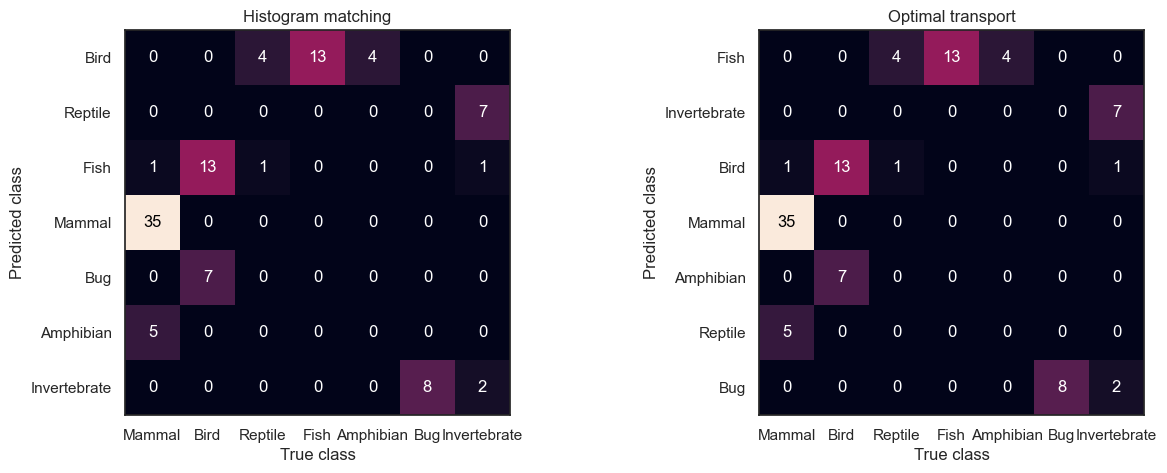
\includegraphics[width=\textwidth]{Attachments/assignment_method.png}
    \caption{Illustration of the two assignment matrices from the different methods after clustering the Zoo dataset. On the left, the naive method and on the right, the optimal assignment method.
    The numbers in the matrices represent the number of samples in the predicted cluster $i$ that are in the true cluster $j$.}
    \label{fig:assignment_methods}
\end{figure}

\begin{table}
\begin{adjustbox}{width=\columnwidth}
\begin{tabular}{lllllll}
\toprule
 &  & \textbf{Runtime (s)} & \textbf{F1} & \textbf{Accuracy} & \textbf{Wasserstein} & \textbf{ARI} \\
Dataset & Method &  &  &  &  &  \\
\midrule
\multirow[t]{6}{*}{\textbf{Zoo}} & \textbf{BOS Random} & 47.28 & 0.77 & 0.78 & 0.35 & \textbf{\underline{0.76}} \\
\textbf{} & \textbf{BOS K-Means} & 4.75 & \textbf{\underline{0.86}} & \textbf{\underline{0.84}} & 0.17 & 0.90 \\
\textbf{} & \textbf{GOD Random} & 52.64 & 0.87 & 0.86 & 0.23 & 0.83 \\
\textbf{} & \textbf{GOD K-Means} & 15.12 & 0.87 & 0.85 & \textbf{\underline{0.14}} & 0.90 \\
\textbf{} & \textbf{K-Means} & \textbf{\underline{0.01}} & 0.70 & 0.64 & 0.84 & 0.58 \\
\textbf{} & \textbf{Gaussian} & 0.75 & 0.79 & 0.76 & 0.33 & 0.73 \\
\cline{1-7}
\multirow[t]{6}{*}{\textbf{Car Evaluation}} & \textbf{BOS Random} & 481.93 & 0.46 & 0.40 & 0.66 & 0.02 \\
\textbf{} & \textbf{BOS K-Means} & 415.80 & 0.42 & 0.37 & 0.73 & -0.01 \\
\textbf{} & \textbf{GOD Random} & 28.95 & 0.43 & 0.40 & 0.41 & -0.04 \\
\textbf{} & \textbf{GOD K-Means} & 19.26 & 0.46 & 0.39 & 0.94 & 0.05 \\
\textbf{} & \textbf{K-Means} & \textbf{\underline{0.01}} & 0.41 & 0.34 & 0.91 & 0.01 \\
\textbf{} & \textbf{Gaussian} & 0.04 & 0.44 & 0.36 & 1.07 & 0.02 \\
\cline{1-7}
\multirow[t]{6}{*}{\textbf{Hayes-Roth}} & \textbf{BOS Random} & 307.60 & 0.37 & 0.39 & 0.25 & 0.00 \\
\textbf{} & \textbf{BOS K-Means} & 101.11 & 0.36 & 0.36 & 0.30 & -0.01 \\
\textbf{} & \textbf{GOD Random} & 11.22 & 0.37 & 0.39 & \textbf{\underline{0.25}} & -0.01 \\
\textbf{} & \textbf{GOD K-Means} & 8.49 & 0.37 & 0.36 & 0.23 & -0.01 \\
\textbf{} & \textbf{K-Means} & \textbf{\underline{0.00}} & 0.34 & 0.33 & 0.16 & -0.01 \\
\textbf{} & \textbf{Gaussian} & 0.02 & \textbf{\underline{0.45}} & \textbf{\underline{0.45}} & 0.11 & \textbf{\underline{0.07}} \\
\cline{1-7}
\multirow[t]{6}{*}{\textbf{Caesarian}} & \textbf{BOS Random} & 52.78 & 0.41 & 0.56 & 0.41 & -0.01 \\
\textbf{} & \textbf{BOS K-Means} & 35.48 & 0.53 & 0.53 & 0.05 & -0.01 \\
\textbf{} & \textbf{GOD Random} & 3.47 & 0.54 & 0.54 & \textbf{\underline{0.04}} & -0.01 \\
\textbf{} & \textbf{GOD K-Means} & 3.51 & 0.59 & 0.59 & 0.09 & 0.02 \\
\textbf{} & \textbf{K-Means} & \textbf{\underline{0.01}} & 0.56 & 0.56 & 0.09 & 0.00 \\
\textbf{} & \textbf{Gaussian} & 0.02 & \textbf{\underline{0.60}} & \textbf{\underline{0.60}} & 0.00 & \textbf{\underline{0.03}} \\
\cline{1-7}
\bottomrule
\end{tabular}
\end{adjustbox}
\caption{
Results of the classification task for the different datasets and the proposed methods. 
The metrics are the F1-score, the accuracy, the Wasserstein distance and the adjusted rand index (ARI). 
The runtime is also reported. 
The best results for each dataset and metric are highlighted in bold and underlined. 
}
\label{tab:results_real}
\end{table}
%\tm{Penser à mettre en avant les bons résultats. Eventuellement ajouter les temps de calcul}

\section{t-SNE plots}
\label{sec:appendix_tsne}
\begin{figure}[H]
    \centering
    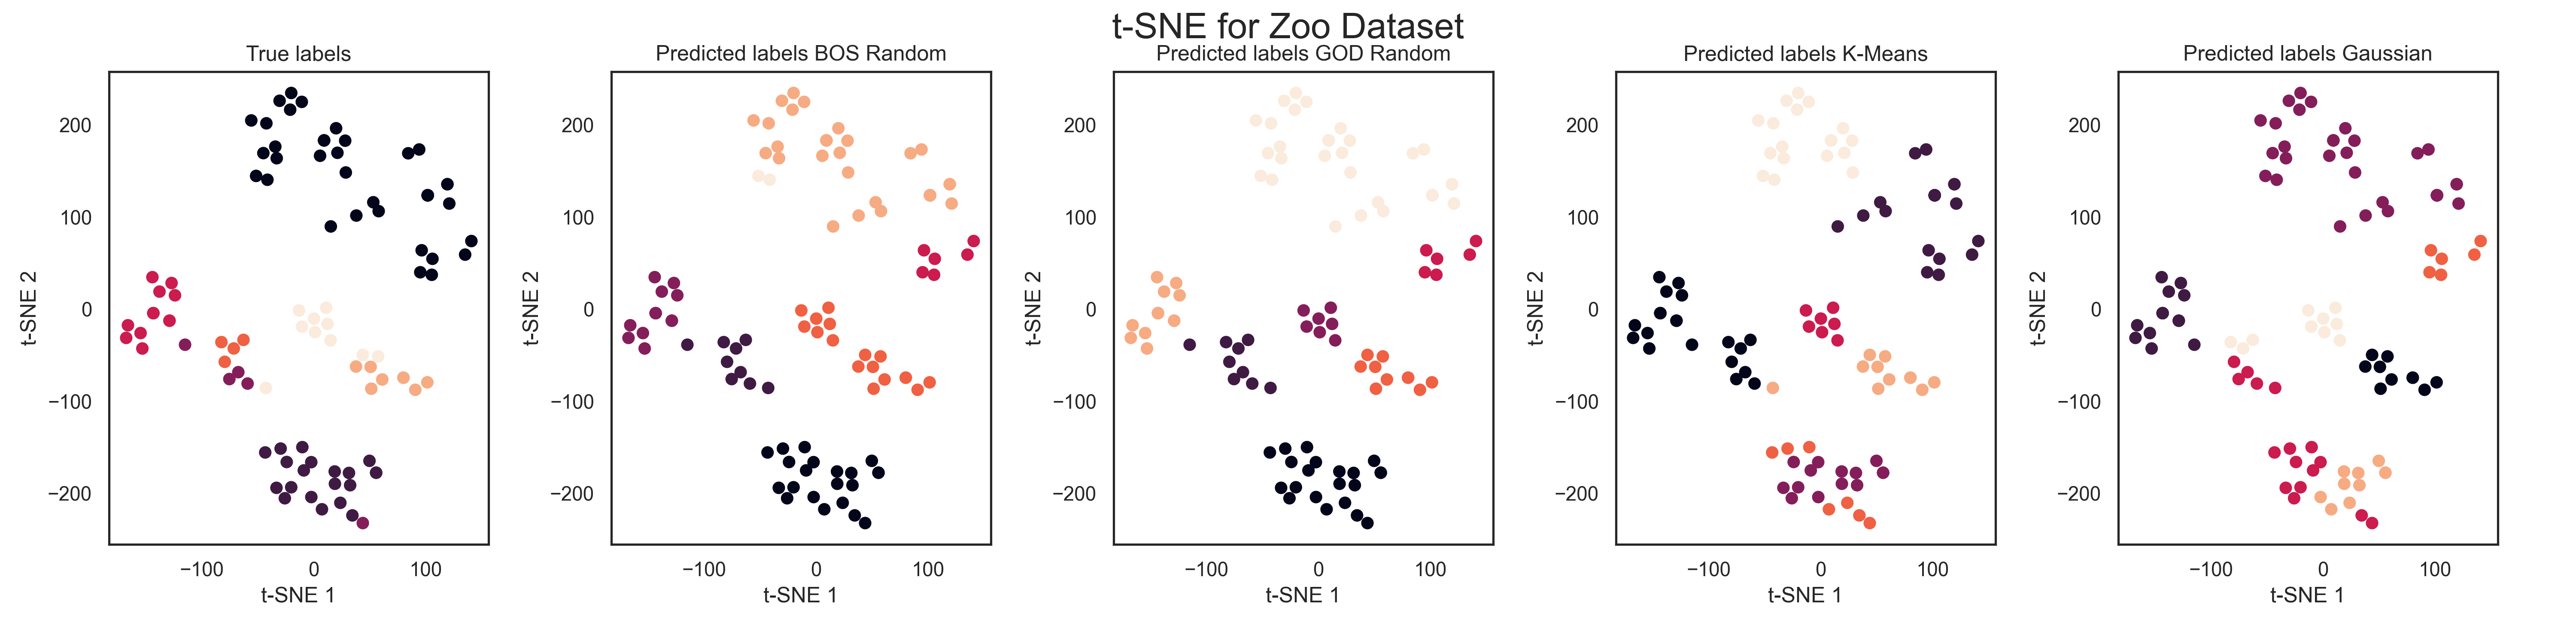
\includegraphics[width=\textwidth]{Attachments/tsne_zoo.png}
    \caption{t-SNE visualization of the Zoo dataset with the true labels and the predicted clusters for the BOS model with random initialization, the GOD model with random initialization, the K-Means algorithm and the Gaussian Mixture Models.}
    \label{fig:tsne_zoo}
\end{figure}

\begin{figure}[H]
    \centering
    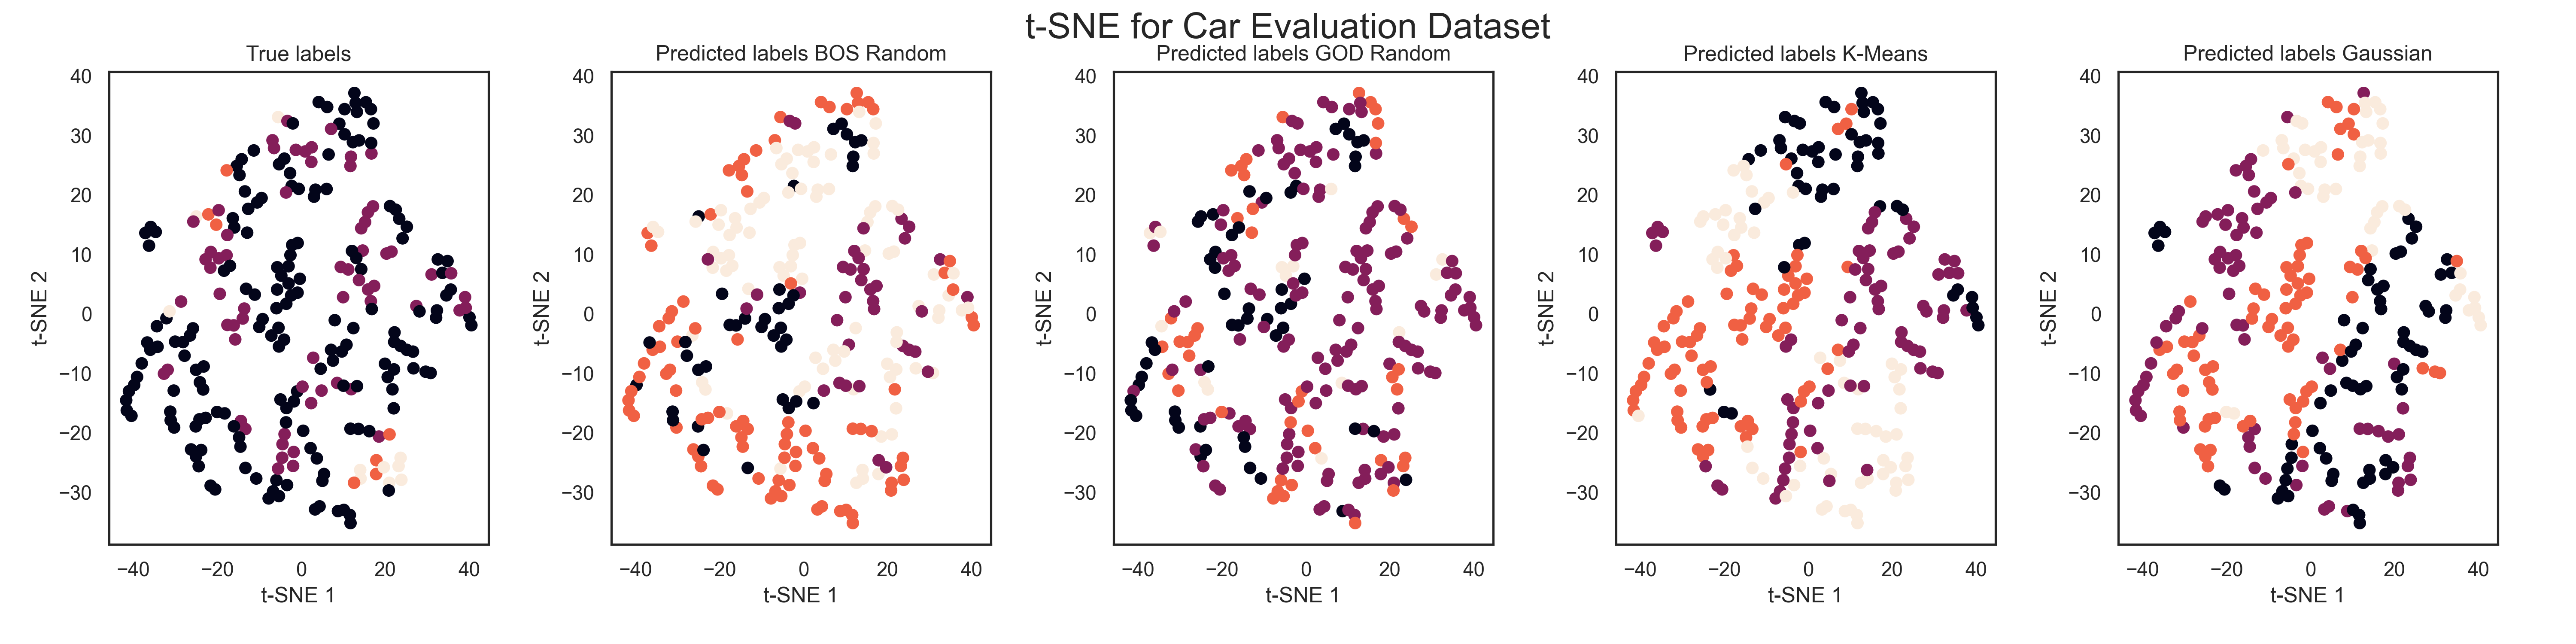
\includegraphics[width=\textwidth]{Attachments/tsne_car_evaluation.png}
    \caption{t-SNE visualization of the Car Evaluation dataset with the true labels and the predicted clusters for the BOS model with random initialization, the GOD model with random initialization, the K-Means algorithm and the Gaussian Mixture Models.}
    \label{fig:tsne_car}
\end{figure}

\begin{figure}[H]
    \centering
    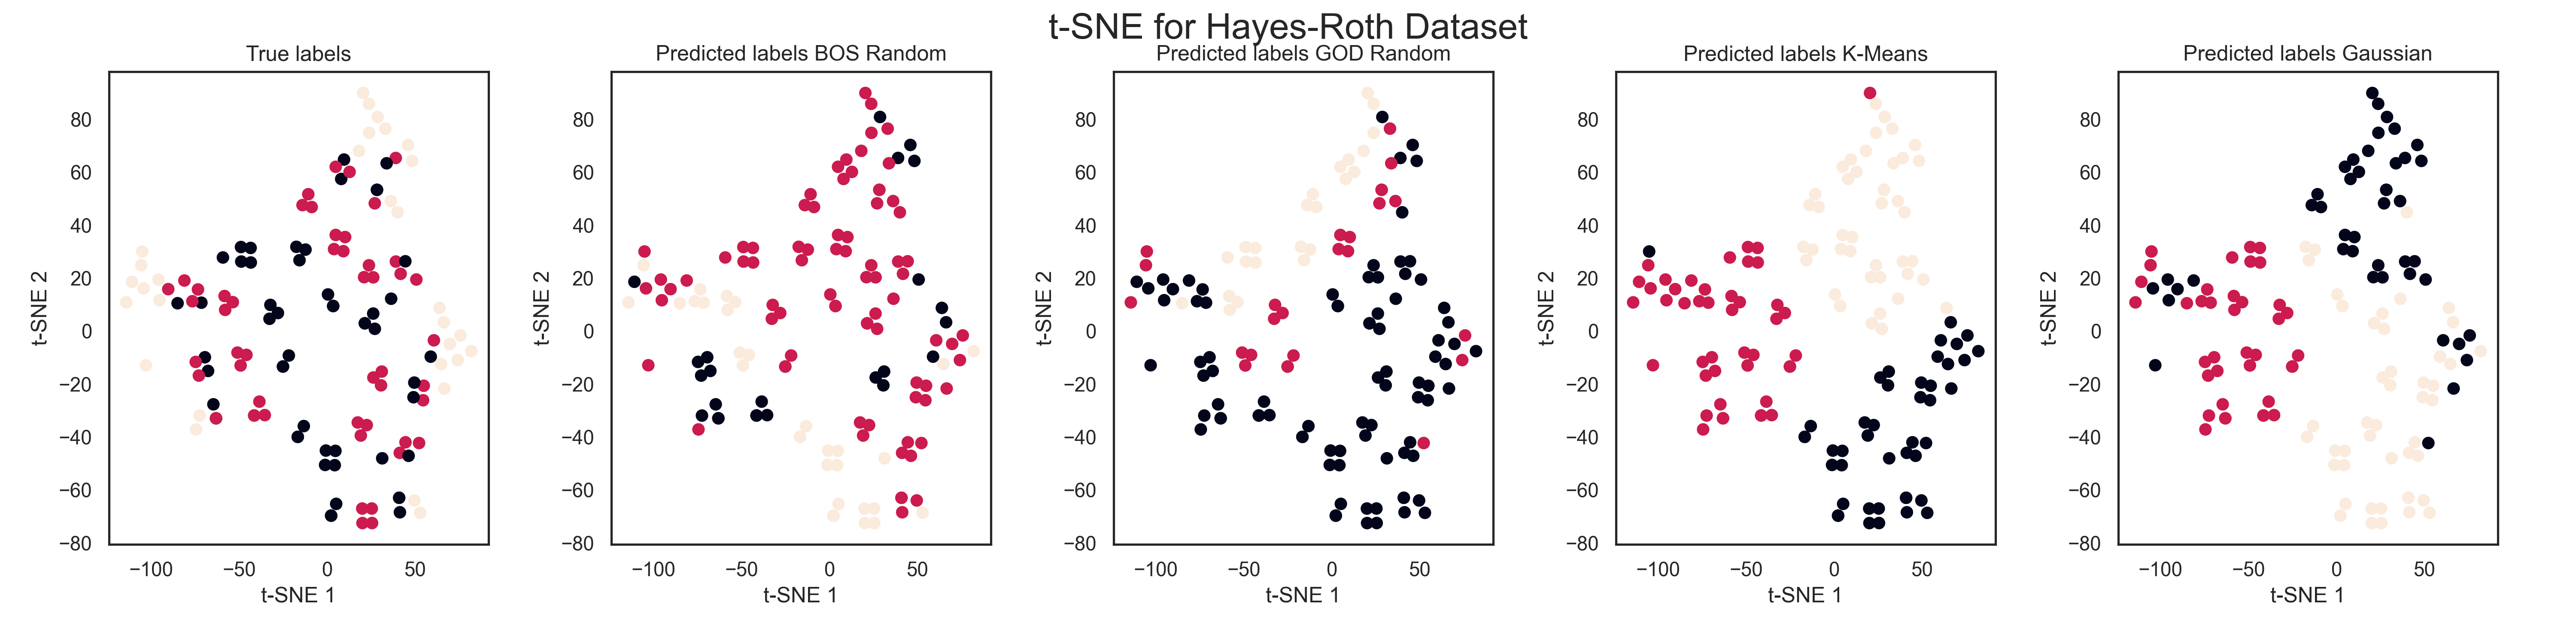
\includegraphics[width=\textwidth]{Attachments/tsne_hayes-roth.png}
    \caption{t-SNE visualization of the Hayes-Roth dataset with the true labels and the predicted clusters for the BOS model with random initialization, the GOD model with random initialization, the K-Means algorithm and the Gaussian Mixture Models.}
    \label{fig:tsne_hr}
\end{figure}

% \begin{figure}[H]
%     \centering
%     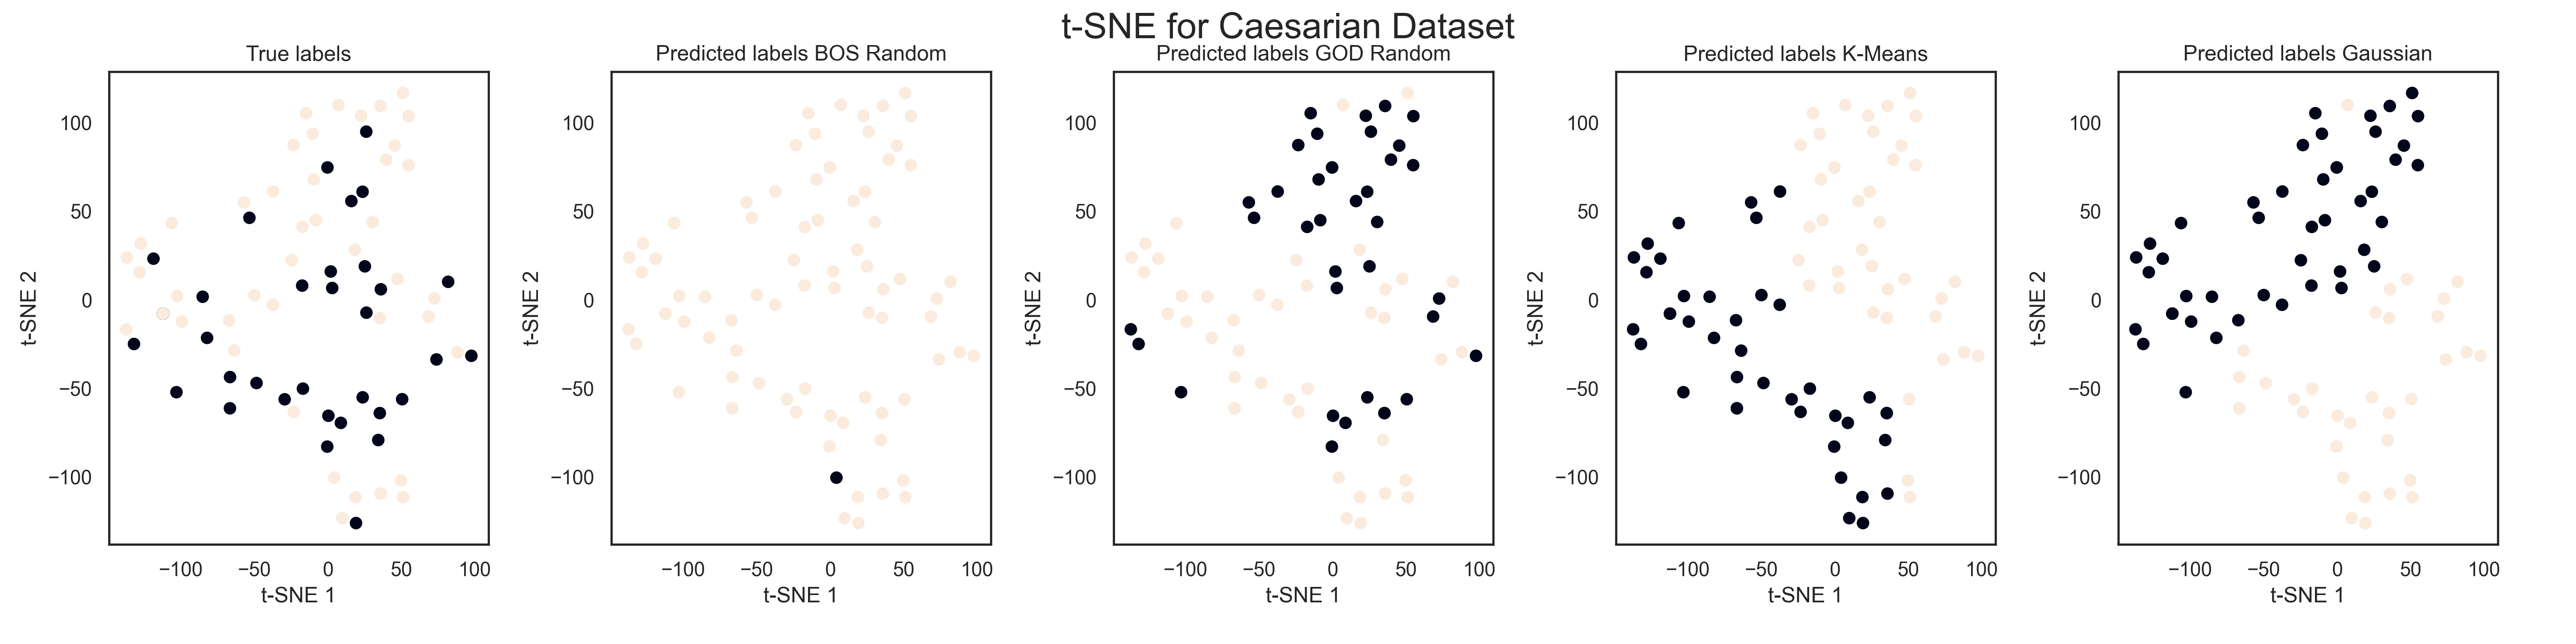
\includegraphics[width=\textwidth]{Attachments/tsne_caesarian.png}
%     \caption{t-SNE visualization of the Caesarian dataset with the true labels and the predicted clusters for the BOS model with random initialization, the GOD model with random initialization, the K-Means algorithm and the Gaussian Mixture Models.}
%     \label{fig:tsne_caesarian}
% \end{figure}

\section{Assignment Matrices}
\label{sec:appendix_assign}

\begin{figure}[H]
    \centering
    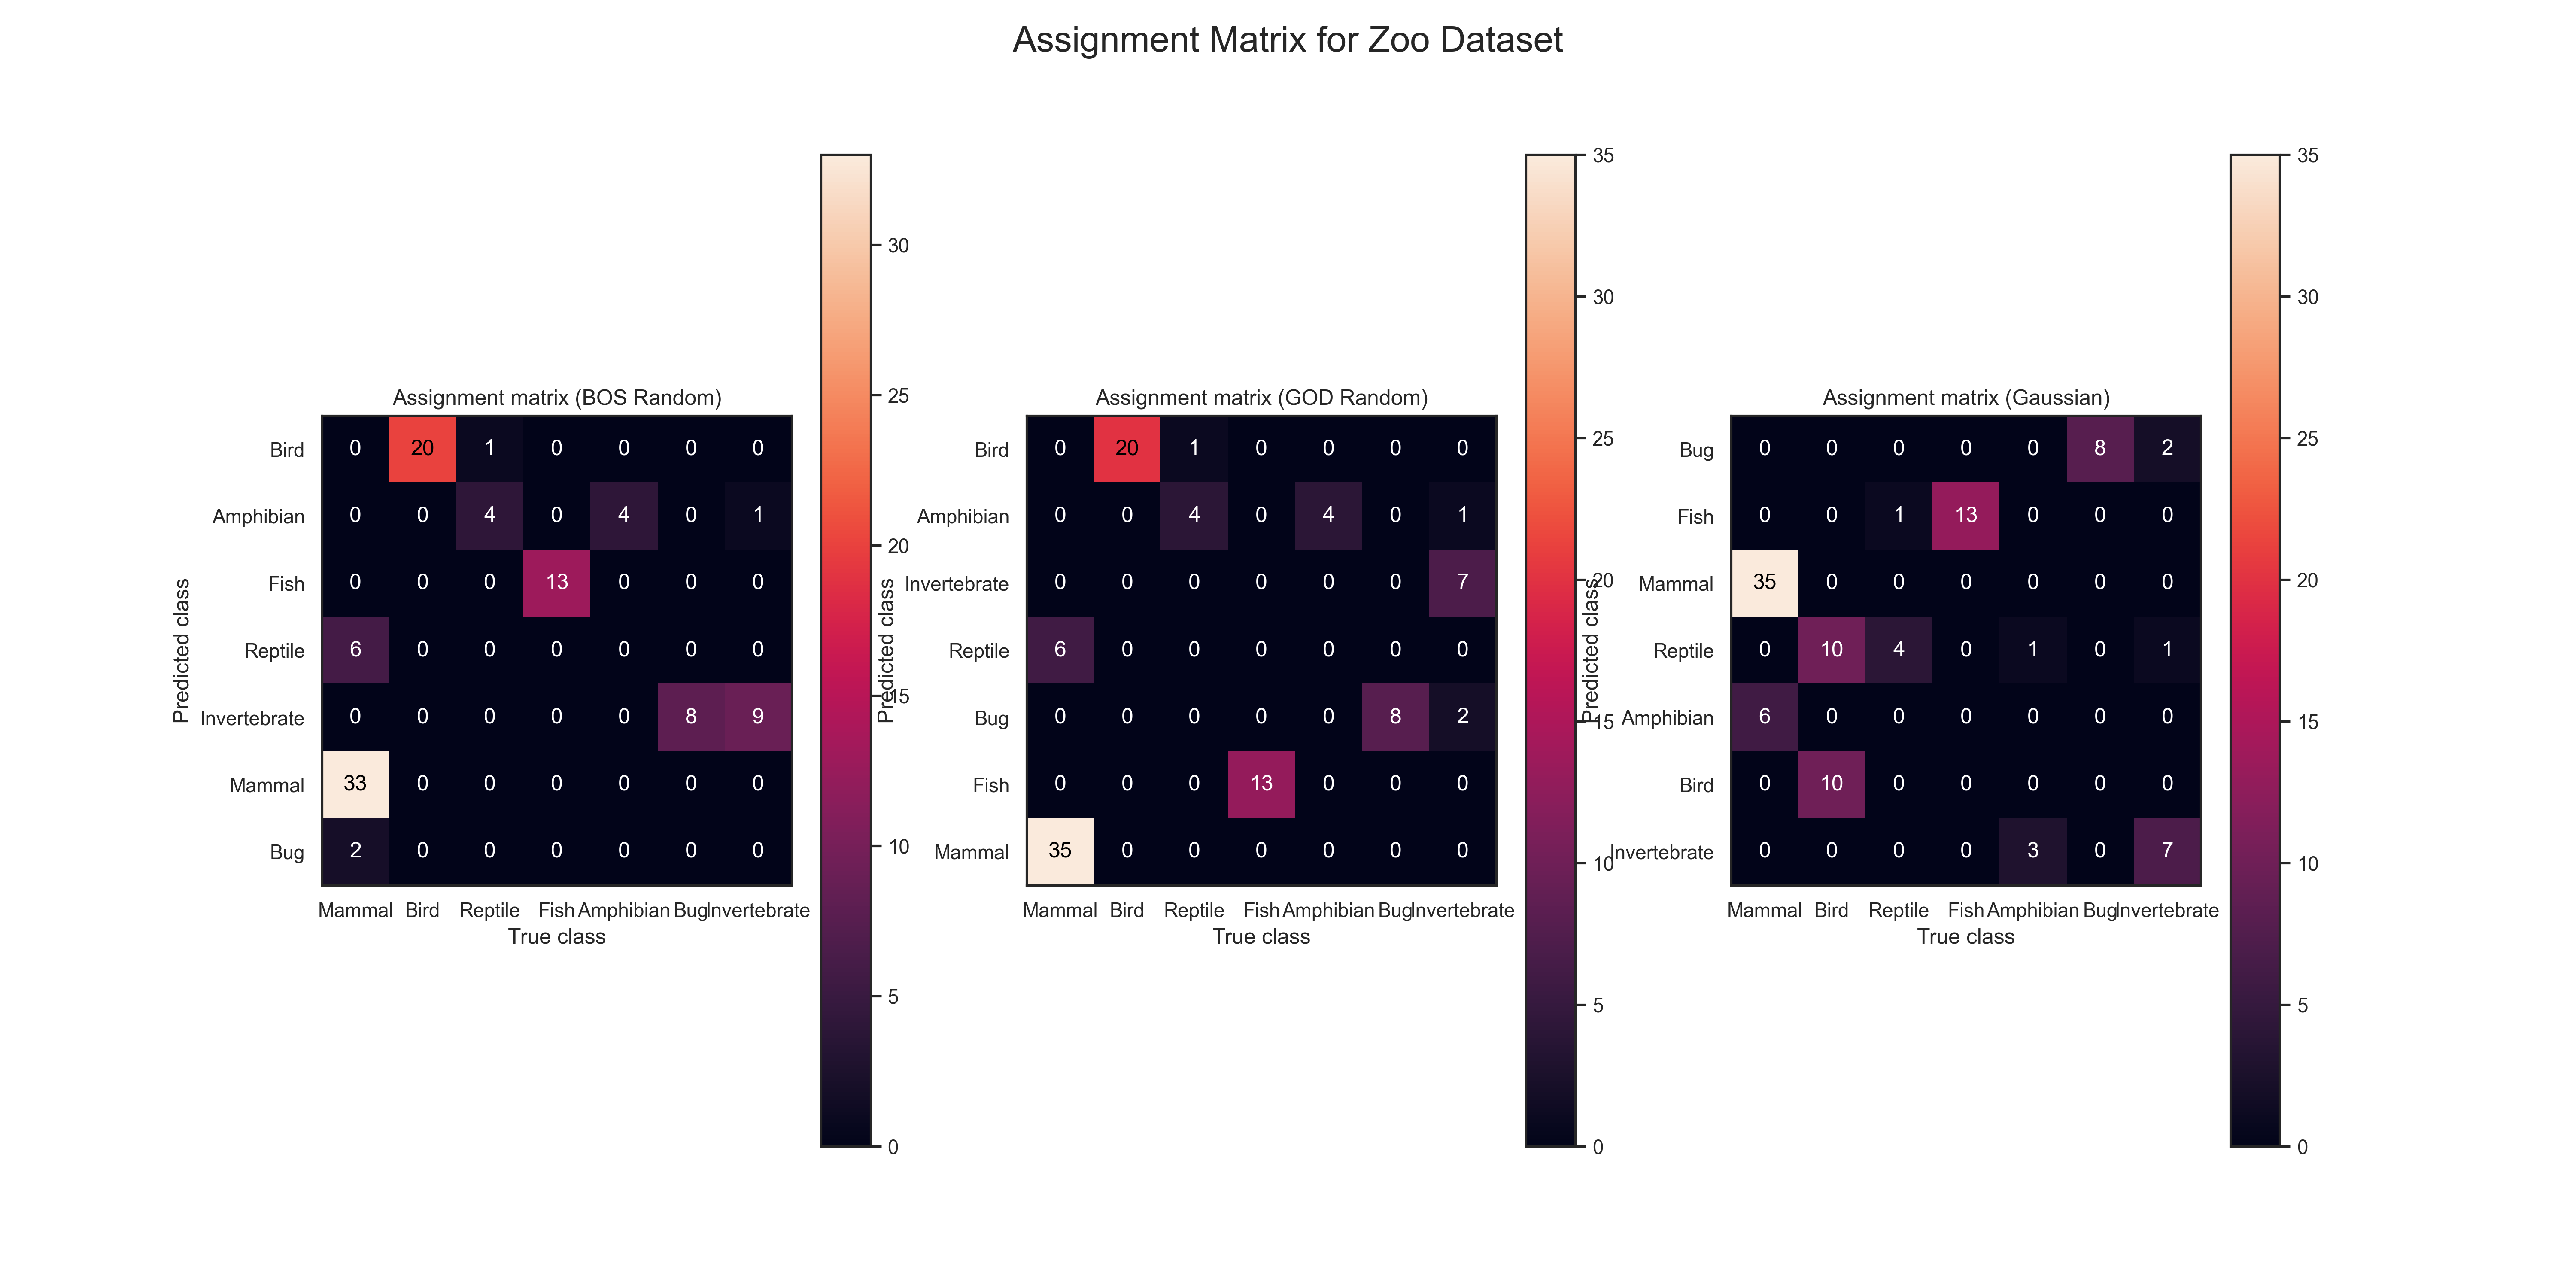
\includegraphics[width=\linewidth]{Attachments/assignment_matrix_zoo.png}
    \caption{Assignment matrix for the Zoo dataset with different methods.}
    \label{fig:assign_zoo}
\end{figure}

\begin{figure}[H]
    \centering
    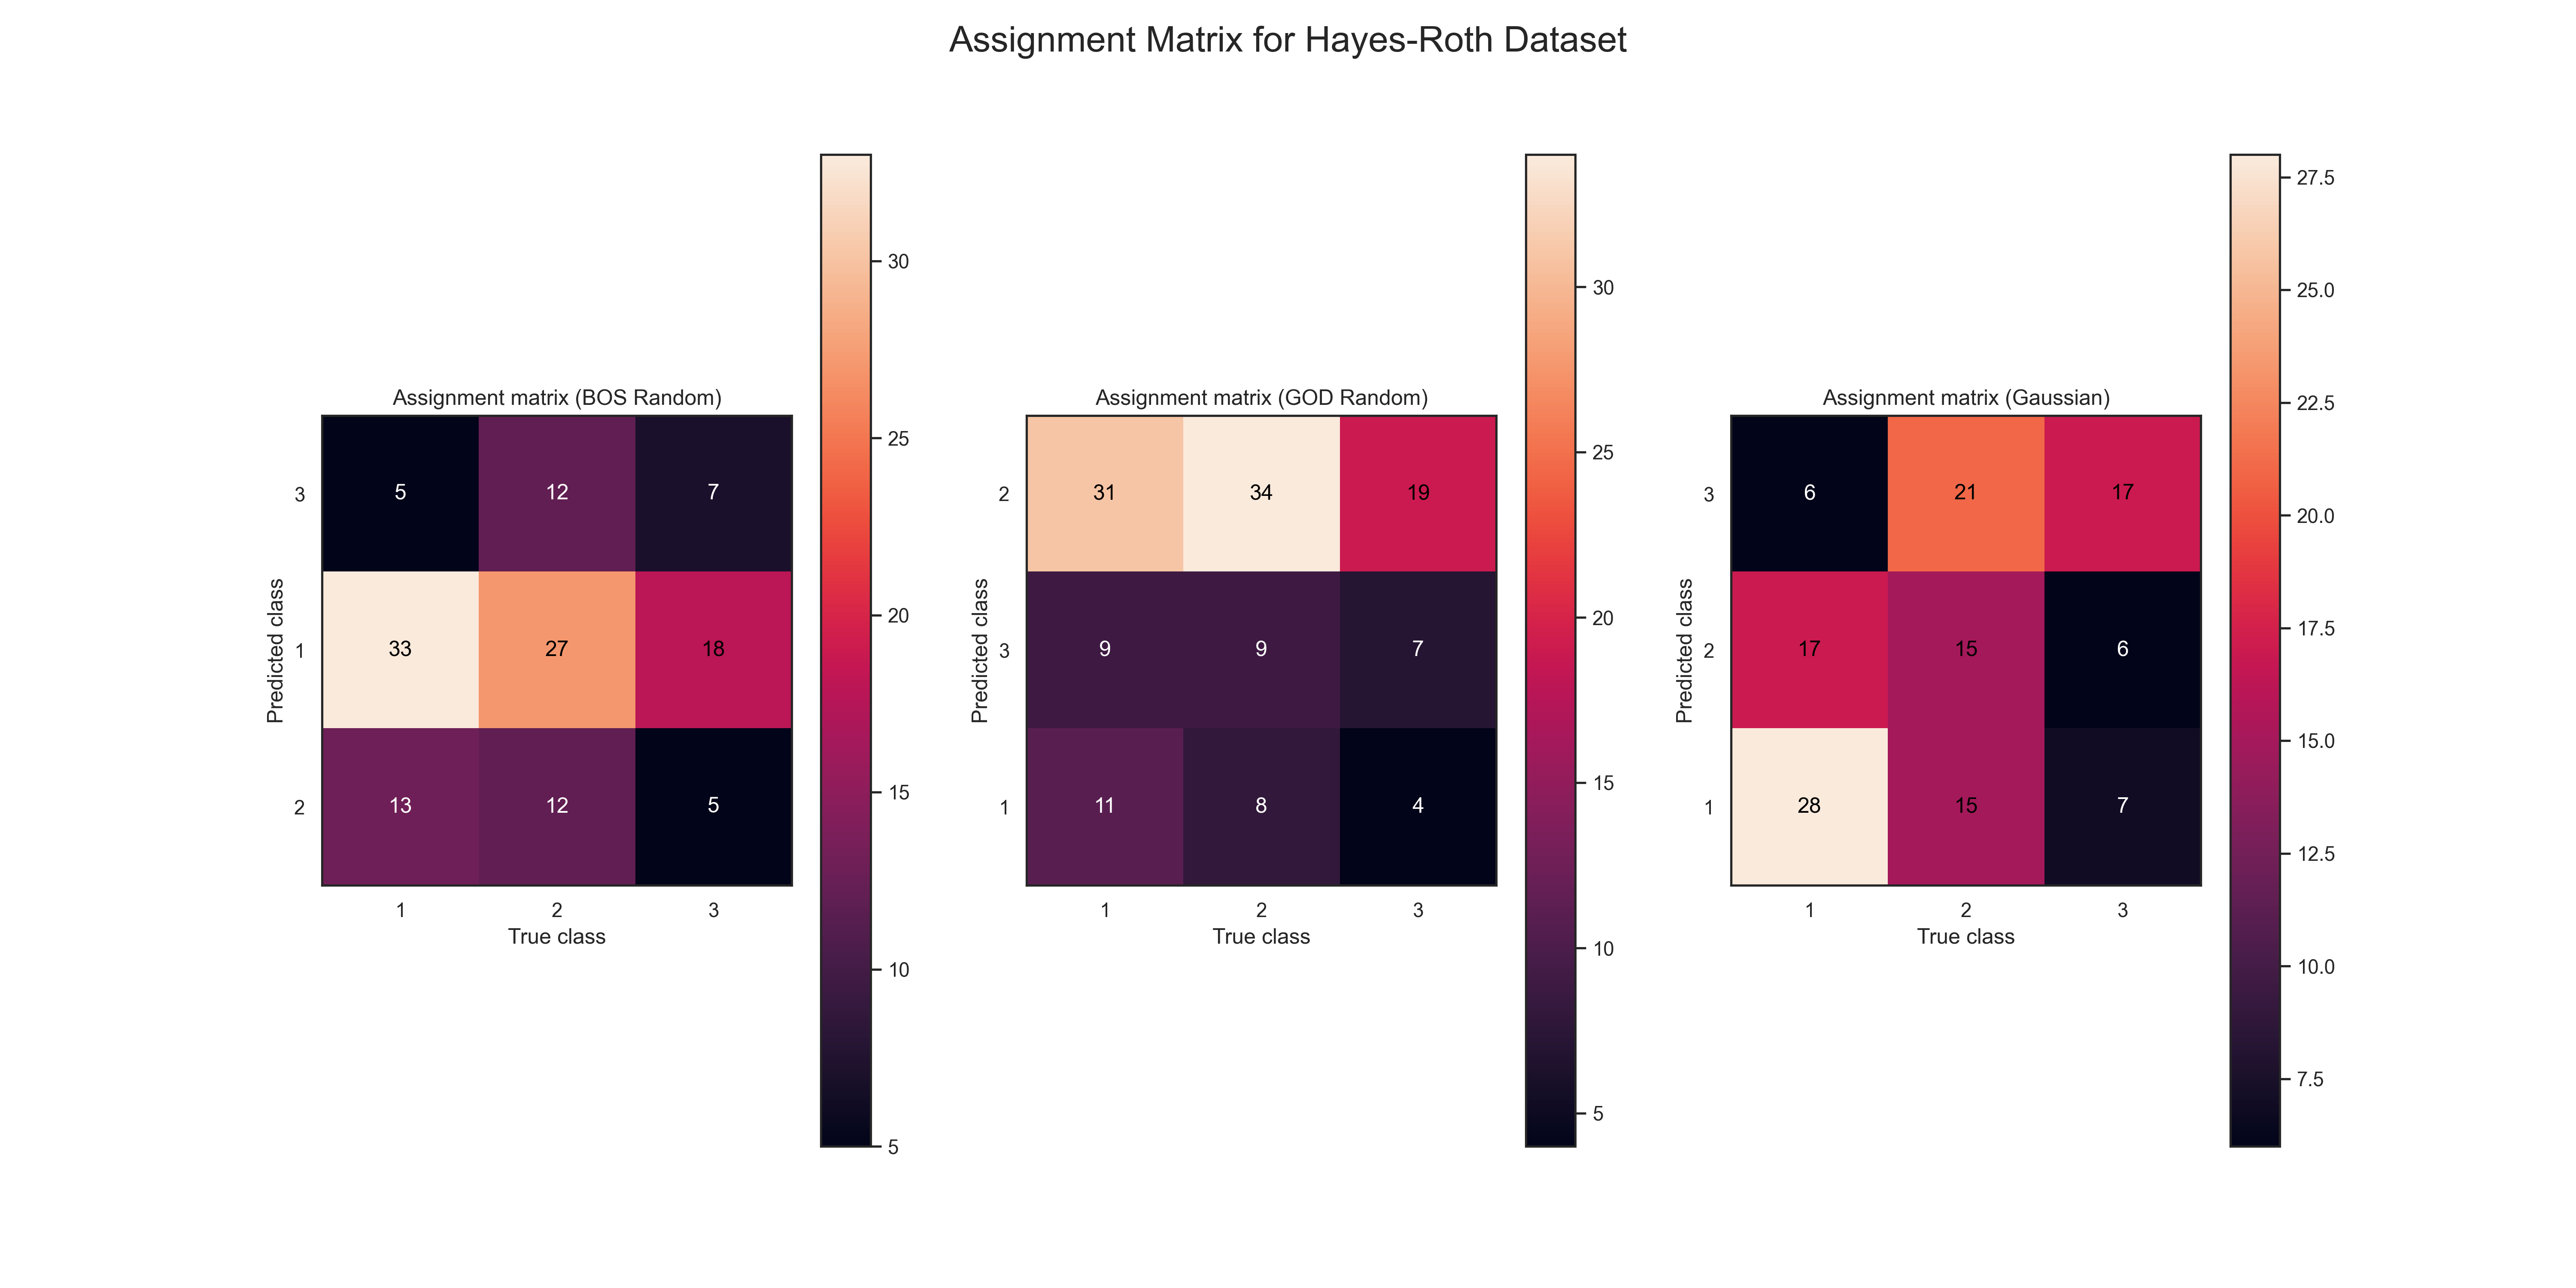
\includegraphics[width=\linewidth]{Attachments/assignment_matrix_hayes-roth.png}
    \caption{Assignment matrix for the Hayes-Roth dataset with different methods.}
    \label{fig:assign_hr}
\end{figure}

\section{Histograms of the different clustering}
\label{sec:appendix_hist}

\begin{figure}[H]
    \centering
    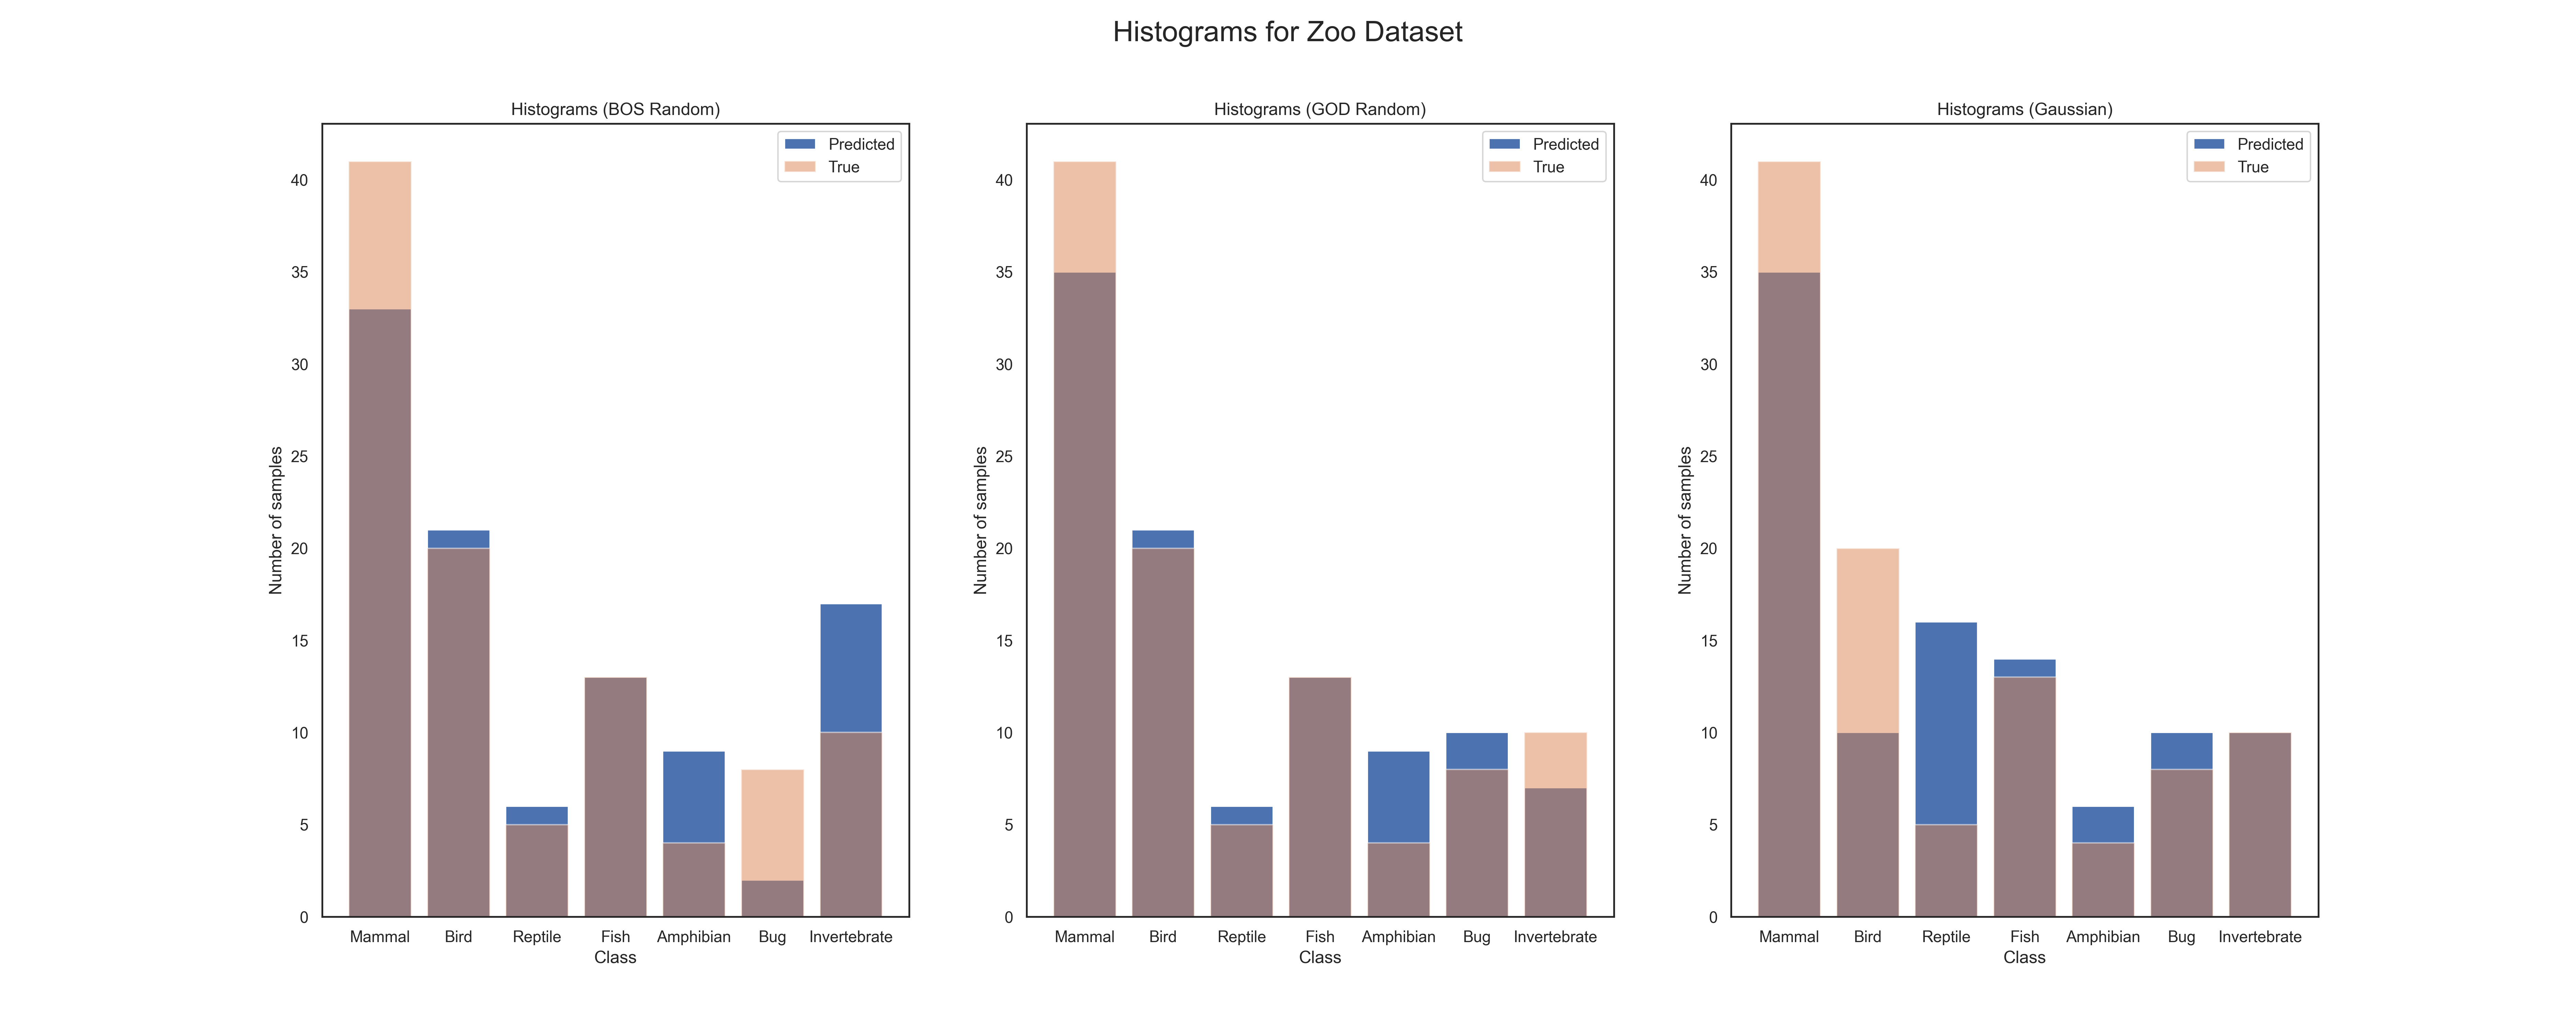
\includegraphics[width=\linewidth]{Attachments/histograms_zoo.png}
    \caption{Histograms for the Zoo dataset with different methods.}
    \label{fig:hist_zoo}
\end{figure}

\begin{figure}[H]
    \centering
    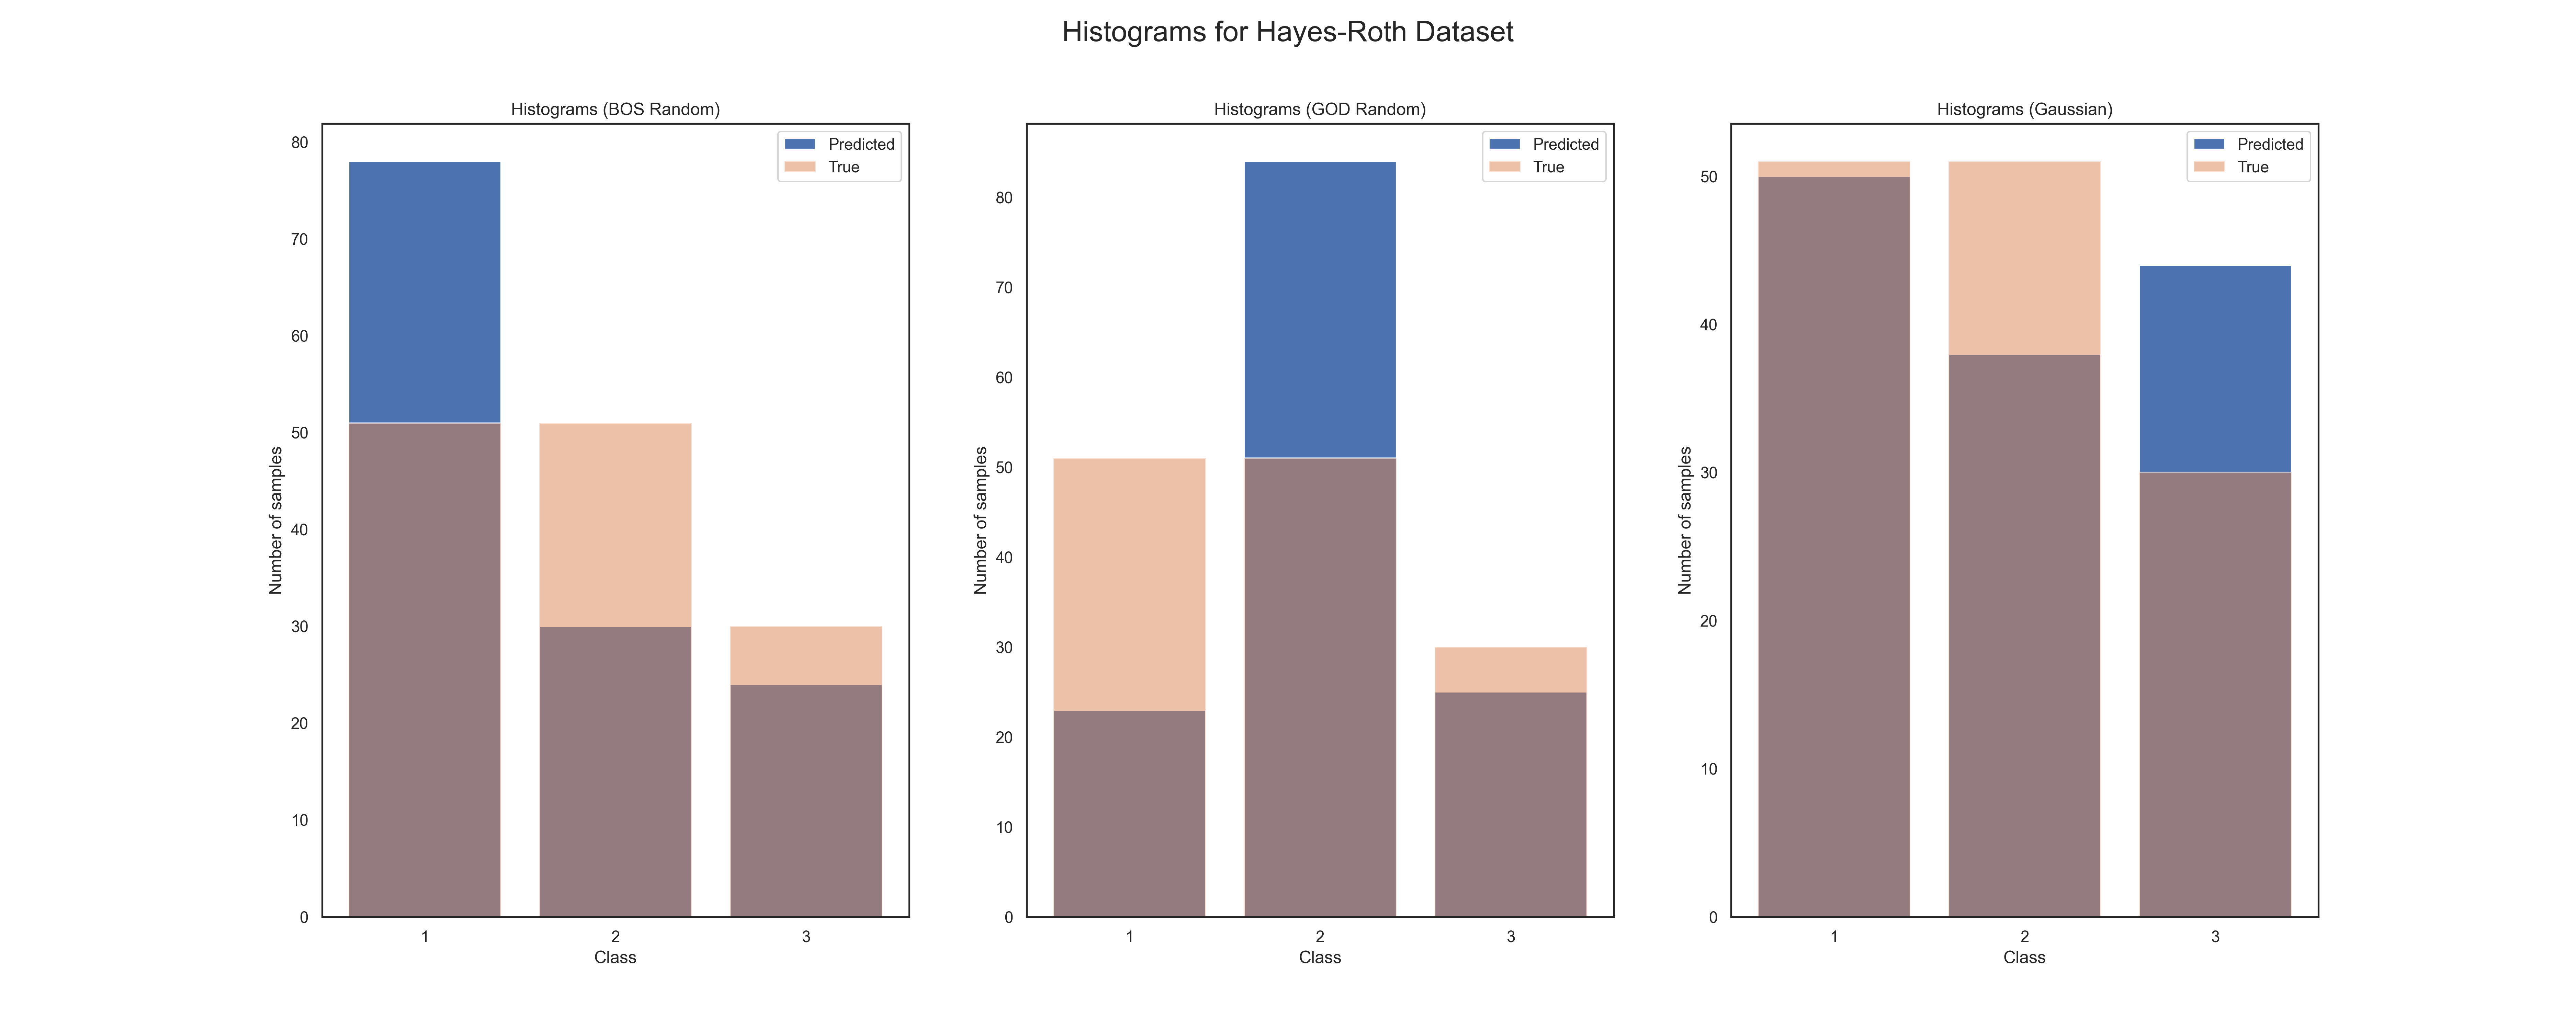
\includegraphics[width=\linewidth]{Attachments/histograms_hayes-roth.png}
    \caption{Histograms for the Hayes-Roth dataset with different methods.}
    \label{fig:hist_hr}
\end{figure}
